% \documentclass[journal]{IEEEtran}
%\documentclass[conference]{IEEEtran} %12pt, draftcls, twocolumn
\documentclass[10pt,twocolumn]{IEEEtran}
\makeatletter
% journal (default) and conference
\def\subsubsection{\@startsection{subsubsection}% name
                                 {3}% level
                                 {\z@}% indent (formerly \parindent)
                                 {0ex plus 0.1ex minus 0.1ex}% before skip
                                 {0ex}% after skip
                             {\normalfont\normalsize\bfseries}}% style
\makeatother
\usepackage[T1]{fontenc}% optional T1 font encoding
%\usepackage{graphicx}
\usepackage{subfigure}
\usepackage{ulem}
\usepackage{amsmath}
\allowdisplaybreaks
\usepackage{hhline}
\usepackage{yfonts,color}
\usepackage{soul,xcolor}
\usepackage{verbatim}
\usepackage{amsmath}
\allowdisplaybreaks
\usepackage{amssymb}
\usepackage{amsthm}
\usepackage{float}
\usepackage{bm}
\usepackage{url}
\usepackage{array}
\usepackage{cite}
\usepackage{graphicx}
\usepackage{tikz}
\usepackage{framed} % for frame
\usepackage{balance} % balance
\usepackage{epsfig,epstopdf}
\usepackage{booktabs}
\usepackage{courier}
\usepackage{subfigure}
\usepackage{pseudocode}
\usepackage{enumerate}
%\usepackage[linesnumbered,ruled]{algorithm2e}
\usepackage{algorithm}
\usepackage{algpseudocode}
\newtheorem{definition}{Definition}
\newtheorem{theorem}{Theorem}
\newtheorem{lemma}[theorem]{Lemma}
\newtheorem{proposition}[theorem]{Proposition}
%\newtheorem{proposition}{Proposition}
\newtheorem{corollary}[theorem]{Corollary}
\newtheorem{assumption}{Assumption}
\newtheorem{remark}{Remark}
\renewcommand{\algorithmicrequire}{\textbf{Initialization:}}  
% Use Input in the format of Algorithm
\renewcommand{\algorithmicensure}{\textbf{Output:}}  
% Use Output in the format of 
\newcommand{\rom}[1]{\uppercase\expandafter{\romannumeral #1\relax}}
\usepackage{color}
\usepackage{soul,xcolor}
\newcommand{\sst}[1]{\st{#1}}
%\newcommand{\sst}[1]{}
%\newcommand{\nm}[1]{}
\newcommand{\nm}[1]{{\color{blue}\bf{[NM: #1]}}}
\newcommand{\bk}[1]{{\color{magenta}{[BK: #1]}}}
\newcommand{\nmmath}[1]{{\color{blue}\text{\bf{[NM: #1]}}}}
\newcommand{\gs}[1]{{\color{orange}\bf{[GS: #1]}}}
\newcommand{\remove}[1]{{\color{magenta}{\bf REMOVE: [#1]}}}
\DeclareMathOperator*{\argmax}{arg\,max}

\usepackage{cancel}
\newcommand\mst[2][red]{\setbox0=\hbox{$#2$}\rlap{\raisebox{.45\ht0}{\textcolor{#1}{\rule{\wd0}{2pt}}}}#2}   


%\newcommand{\nm}[1]{}
%\newcommand{\sst}[1]{}
%\newcommand{\gs}[1]{}
%\newcommand{\remove}[1]{}
\newcommand{\add}[1]{{\color{red}{#1}}}
\newcommand{\ull}[1]{\textbf{\color{red}\ul{#1}}}
%\pagestyle{empty}
\normalem
\title{Utility Maximization in Cognitive Radio Networks using POMDP Approximate Value Iteration methods}
\author{Bharath Keshavamurthy, Nicol\`{o} Michelusi
\thanks{This research has been funded by -----.}
\thanks{The authors are with the School of Electrical and Computer Engineering, Purdue University. email: \{bkeshava,michelus\}@purdue.edu.}
%\vspace{-12mm}
}
\begin{document} 
\setulcolor{red}
\setul{red}{2pt}
\maketitle
\setstcolor{red}
\begin{abstract}
Cognitive radio technologies will be critical to the wireless communication infrastructure in the near future due to the increasingly incredible number of applications being added to the computer networking ecosystem, both in the commercial and the military spheres, resulting in increased pressure on the available spectrum which is a limited physical resource. In this paper, we propose a novel channel access strategy in networks with multiple licensed users wherein a cognitive radio node should learn the correlation model defining the occupancy behavior of the incumbents and devise an optimal strategy based on this correlation model by solving a utility maximization problem in a partially observable radio environment setting. Since the computational complexity associated with solving for the optimal channel access strategy scales exponentially with the number of spectrum bands under consideration, we propose a system employing approximate POMDP value iteration methods, namely, the PERSEUS algorithm. Furthermore, through system simulations, we compare the performance of standard MAP-based state estimators and correlation-coefficient based clustering algorithms in the state-of-the-art against our proposed system employing a customized PERSEUS algorithm, with respect to the secondary network throughput and the number of collisions with the incumbent transmissions.
\end{abstract}
\begin{IEEEkeywords}
Hidden Markov Model, POMDP, and the PERSEUS Algorithm
\end{IEEEkeywords}
\section{Introduction}
With the advent of fifth-generation wireless communication networks, the problem of spectrum scarcity has been exacerbated. For some time now, cognitive radio technologies have been in the spotlight as a potential solution to this problem in commercial and military applications. Cognitive radio networks facilitate efficient spectrum utilization by intelligently accessing "white spaces" left unused by the sparse and infrequent transmissions of the licensed users. By intelligently accessing these spatial and temporal spectrum holes, the radio nodes in a cognitive radio network complete their allotted network flows subject to QoS requirements while ensuring that their transmission do not interfere with the incumbents in the network. This poses an interesting optimization problem of maximizing secondary network throughput while complying with strict non-interference with the transmissions of the primary, licensed users. A crucial aspect underlying the design of cognitive radio networks is the channel access protocol in the MAC layer of the stack. In this regard, the current state-of-the-art involves channel access strategies dictated by multi-armed bandits, reinforcement learning agents, and other custom heuristics. However, almost all these works assume independence among channels in the discretized spectrum which is imprudent because licensed users exhibit both spatial and temporal correlation in their channel occupancy behavior: the primary users frequently occupy a set of adjacent channels implying that these channels would then be correlated spatially with respect to the occupancy behavior of a particular incumbent and furthermore, the primary users frequently use the same set of channels across time which further implies that these channels are correlated temporally. This pattern in occupancy behavior of the incumbents imputes very high levels of correlation among channels which need to be leveraged for more accurate predictions of spectrum holes in order to satisfy the QoS guarantees of flows in the secondary network while limiting collisions with incumbent transmissions. In this paper, we propose techniques to exploit the correlation model underlying the occupancy behavior of incumbents in the network- a parameter estimation algorithm to learn the aforementioned correlation model, a state estimation algorithm to infer channel occupancy from noisy and incomplete information, and an approach to solve for the optimal channel sensing and access policy to be followed by the cognitive radio node. We define the signal model in Section II of this document followed by the formulations, approaches, and algorithms for each of the three interconnected sub-problems detailed earlier, in Section III, and finally, in Section IV of this document, we present an evaluation of the system along with comparisons with other approaches in the state-of-the-art.
\\\bk{Include a brief description of the approaches in a few papers in the state-of-the-art: the correlation coefficient based paper, restless MABs, and SARSA}
\section{System Model}
\begin{figure}
    \centering
    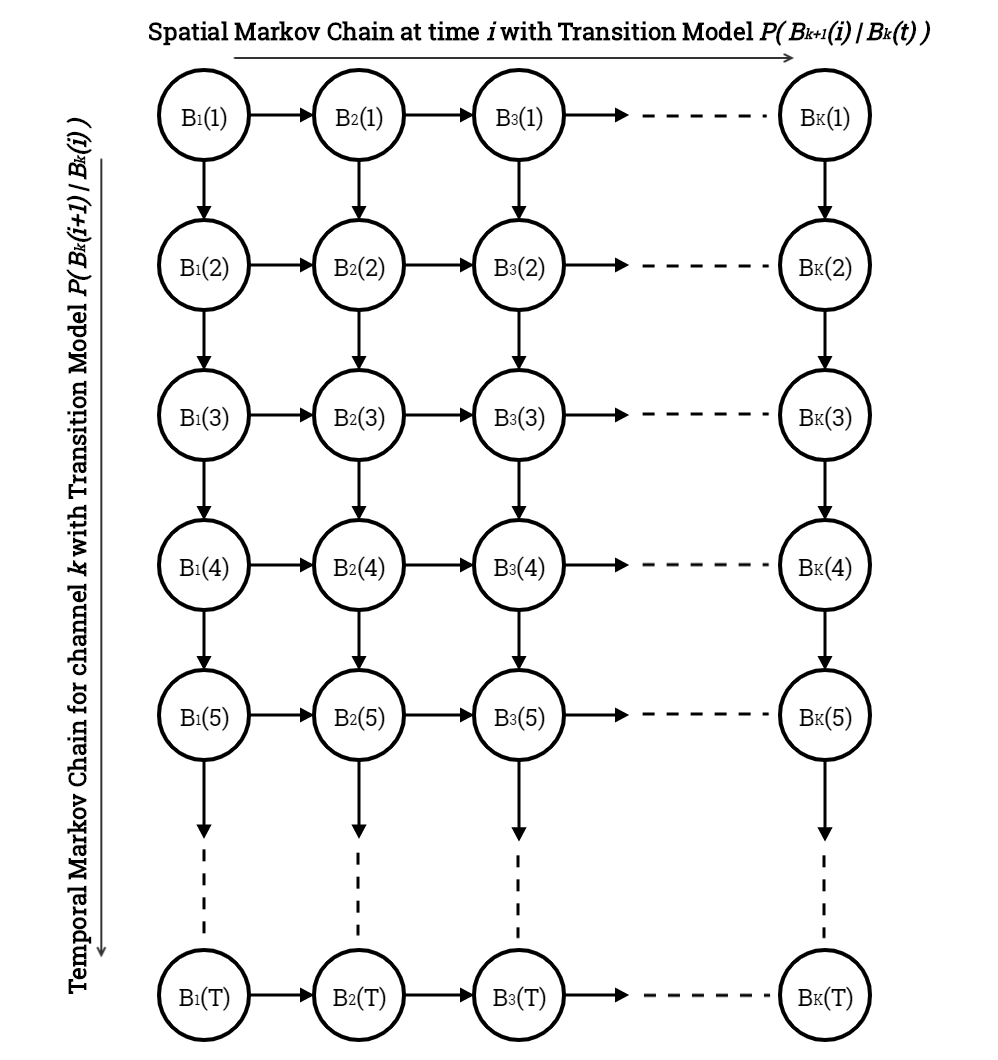
\includegraphics[scale=0.252]{minerva_occupancy_markov_chain.png}
    \caption{The correlation model across channels and across time indices underlying the occupancy behavior of incumbents in the network
    \nm{why do you call it "spatial" Markov chain?}}
    \label{fig:Figure 1}
\end{figure}
\subsection{Signal Model}\label{A}
We consider a network consisting of $P$ licensed users termed the Primary Users (PUs) and one cognitive radio node termed the Secondary User (SU) equipped with a spectrum sensor. The objective of the SU is to opportunistically access portions of the spectrum left unused by the PUs in order to maximize its own throughput. To this end, the SU should learn how to intelligently access spectrum holes (white-spaces) intending to maximize its throughput while maintaining strict non-interference compliance with incumbent transmissions.
The wideband signal received at the SU receiver at time $n$ is denoted as $y(n)$ and is given by 
\begin{equation}\label{1}
    y(n)\ =\ \sum_{p=1}^{P}\sum_{l=0}^{L_{p}-1} h_{p}(l)x_{p}(n-l) + v(n),
\end{equation}
where $y(n)$ is expressed as a convolution of the signal $x_{p}(n)$ of the $p$th PU with the channel impulse response $h_{p}(n)$, and $v(n)$ denotes additive white Gaussian noise (AWGN) with variances $\sigma_v^2$. Eq. (\ref{1}) can be written in the frequency domain by taking a $K$-point DFT which decomposes the observed wideband signal into $K$ discrete narrow-band components as 
\begin{equation}\label{2}
    Y_k(i)\ =\ \sum_{p=1}^{P}H_{p,k}(i)X_{p,k}(i)+V_k(i),
\end{equation}
\nm{Are PUs using OFDMA? Note that this signal model makes sense only in the OFDM context.}
where $i \in \{1,2,3,\dots,T\}$ represents the time index; $k \in \{1,2,3,\dots,K\}$ represents the index of the components in the frequency domain; $V_k(i) \sim \mathcal{CN}(0,\sigma_V^2)$ represents a circularly symmetric additive complex Gaussian noise sample, i.i.d across channel\nm{frequency?} indices and across time indices; $X_{p,k}(i)$ is the signal of the $p$th PU in the frequency domain, and $H_{p,k}(i)$ is its frequency domain channel. The noise samples are assumed to be independent of the occupancy state of the channels. We further assume that the $P$ PUs employ an orthogonal access to the spectrum (e.g., OFDMA) so that $X_{p,k}(i)X_{q,k}(i)=0,\ \forall p\neq q$. Thus, letting $p_k$ be the index of the PU that contributes to the signal in the $k$th spectrum band (possibly, $p_k=0$ if no PU is transmitting in the $k$th spectrum band), and letting  $H_{k}(i)=H_{p_k,k}(i)$ and $X_{k}(i)=X_{p_k,k}(i)$, we can rewrite \eqref{2} as 
\begin{equation}\label{3}
    Y_k(i)\ =\ H_{k}(i)X_{k}(i) + V_k(i).
\end{equation}
Thus, $H_k(i)$ represents the $k$th DFT coefficient of the impulse response $h_{p_k,k}(n)$ of the channel in between the PU operating on the $k$th spectrum band and the SU, at time $i$; we model it as a zero-mean circularly symmetric complex Gaussian random variable with variance $\sigma_H^2$, $H_k \sim \mathcal{CN}(0,\sigma_H^2)$, i.i.d. across frequency bands, over time, and independent of the occupancy state of the channels.
\subsection{PU Spectrum Occupancy Model}
We now introduce the model of PU occupancy over time and across the frequency domain. We model each $X_k(i)$ as 
\begin{equation}\label{4}
    X_k(i)=\sqrt{P_{tx}}B_k(i)S_k(i),
\end{equation}
where $P_{tx}$ is the transmission power of the PUs, $S_k(i)$ is the transmitted symbol modelled as a constant amplitude signal, $|S_k(i)|=1$, i.i.d. over time and across frequency bands; \footnote{In the case where $S_k(i)$ does not have constant amplitude, we may approximate $H_{k}(i)S_{k}(i)$ as complex Gaussian with zero mean and variance $\sigma_H^2\mathbb E[|S_{k}(i)|^2]$, without any modification to the subsequent analysis.} $B_k(i)\in\{0,1\}$ is the binary spectrum occupancy variable, with $B_k(i)=1$ if the $k$th spectrum band is occupied by a PU at time $i$, and $B_k(i)=0$ otherwise. Therefore, the PU occupancy behavior in the entire wideband spectrum of interest at time $i$, discretized into narrow-band frequency components can be modeled as the vector 
\begin{equation}\label{5}
    \vec{B}(i)\ =\ [B_1(i),B_2(i),B_3(i),\cdots,B_K(i)]^T \in \{0,1\}^K.
\end{equation}
PUs join and leave the spectrum at random times. To capture this temporal correlation in the spectrum occupancy dynamics of PUs, we model the spectrum occupancy dynamics as a Markov process: given $\vec{B}(i)$, the spectrum occupancy state at time index $i$, $\vec{B}(i+1)$ is independent of the past, $\vec{B}(j),\ j < i$; $j, i \in \{1,2,3,\dots,T\}$, i.e. 
\begin{equation}\label{6}
    \begin{aligned}
        \mathbb{P}(\vec{B}(i+1)|\vec{B}(j),\ \forall j \leq i)\ =\ \mathbb{P}(\vec{B}(i+1)|\vec{B}(i)).
    \end{aligned}
\end{equation}
Additionally, when joining the spectrum pool, PUs occupy a number of adjacent spectrum bands, and may vary their spectrum needs depending on traffic demands, channel conditions, etc. To capture this behavior, we model $\vec{B}(i)$ as having Markovian correlation across the bands as, 
\begin{align}\label{7}
&         \mathbb{P}(\vec{B}(i+1)|\vec{B}(i))\\&=
\nonumber
         \mathbb{P}(B_{1}(i+1)|B_{1}(i))
         \prod_{k=2}^{K}\ \mathbb{P}(B_{k}(i+1)|B_{k}(i),B_{k-1}(i+1)).
\end{align}
That is, the spectrum occupancy at time $i+1$ in frequency band $k$, $B_{k}(i+1)$, depends on the  occupancy state of the adjacent spectrum band at the same time, $B_{k-1}(i+1)$, and that of the same spectrum band $k$ in the previous time index $i$, $B_{k}(i)$.
\nm{as shown in Fig. XXX}

\subsection{Spectrum Sensing Model}
In order to detect the available spectrum holes, the SU performs spectrum sensing. However, owing to physical design limitations at the SU's spectrum sensor \nm{citation?}, not all channels in the discretized spectrum can be sensed \add{at once}. Therefore, due to limited sensing capabilities, the SU can sense only $\kappa$ out of $K$ spectrum bands at any given time, with $1\leq \kappa\leq K$. Let $\mathcal K_{i}\subseteq\{1,2,\dots,K\}$ with $|\mathcal K_i|\leq \kappa$ be the set of indices corresponding to the spectrum bands sensed by the SU at time $i$, which is part of our design.\sst{ Then, we model the emission process of the HMM as }
\nm{you mention HMM but you did not introduce it yet. I would say instead:}
\add{Then, we define the observation vector}
\begin{equation}\label{8}
    \vec{Y}(i)\ =\ [Y_k(i)]_{k\in\mathcal K_i},
\end{equation}
where $Y_k(i)$ is given by \eqref{3}.
The true states $\vec{B}(i)$ encapsulate the actual occupancy behavior of the PU and the measurements at the SU are noisy observations of these true states which are modeled to be the observed states of a Hidden Markov Model (HMM). Given the spectrum occupancy vector $\vec{B}(i)$ and the set of sensed spectrum bands $\mathcal K_i$, the probability density function of $\vec{Y}(i)$ is expressed as
\begin{equation}\label{9}
    f(\vec{Y}(i)|\vec{B}(i),\mathcal K_i)=\prod_{k\in\mathcal K_i}f(Y_k(i)|B_k(i)),
\end{equation}
owing to the independence of channels, noise, and transmitted symbols across frequency bands. Moreover, \add{from \eqref{3} we find that}
\begin{equation}\label{10}
 Y_k(i)|B_k(i)\sim \mathcal{CN}(0,\sigma_H^2P_{tx}B_k(i)+\sigma_V^2).
\end{equation}
\nm{moved to next sec.}
\sst{Now, we model the spectrum access scheme of the SU as a Partially Observable Markov Decision Process (POMDP) wherein the goal of the POMDP agent is to devise an optimal sensing and access policy in order to maximize its throughput while maintaining strict non-interference compliance with incumbent transmissions.}
\subsection{POMDP Agent Model}
\add{In this section, we model the spectrum access scheme of the SU as a Partially Observable Markov Decision Process (POMDP) wherein the goal of the POMDP agent is to devise an optimal sensing and access policy\nm{are you optimizing also the spectrum access decision, or only the spectrum sensing?} in order to maximize its throughput while maintaining strict non-interference compliance with incumbent transmissions.}
\add{In fact,} the agent's limited sensing capabilities coupled with its noisy observations result in an increased level of uncertainty at the agent's end about the occupancy state of the spectrum under consideration and the exact effect of executing an action on the radio environment. The transition model of the underlying MDP as described by \eqref{7}, is denoted by $A$\nm{use $\mathbf P$ instead} and is learnt by the agent by interacting with the radio environment. The emission model is denoted by $M$ and is given by \eqref{9}, with $f(Y_k(i)|B_k(i))$ given by \eqref{10}. We model the POMDP as a tuple $(\mathcal B,\mathcal{A},\mathcal{Y},A,M)$ where $\mathcal{B}\equiv\{0,1\}^K$ represents the state space of the underlying MDP with states $\vec{B}$ given by all possible realizations of the spectrum occupancy vector as described by \eqref{3}, $\mathcal{A}$ represents the action space of the agent, given by all $\left(\begin{array}{c}K\\\kappa\end{array}\right)$ possible combinations in which the $\kappa$ spectrum bands are chosen to be sensed out of $K$ at any given time; and $\mathcal{Y}$ represents the observation space of the agent based on the signal model outlined in the previous subsection. 

\add{The state of the POMDP at time $i$ is given by the \emph{prior belief} $b_i$,\nm{notation: you use $B$ for spectrum occupancy, use something different for belief. $\beta$?}
which represents the probability distribution of the underlying MDP state $\vec{B}(i)$, given the information collected by the agent up to time $i$, but before collecting the new information in slot $i$}
At the beginning of each time index $i$, \add{given $b_i$,} the agent selects $\kappa$ spectrum bands out of $K$ \add{according to a policy $\mu(b_i)$}, thus defining the sensing set $\mathcal K_i$, performs spectrum sensing  on these spectrum bands, observes $\vec{Y}(i)\in \mathcal{Y}$, and updates its \emph{\add{posterior} belief} of the current spectrum occupancy $\vec{B}(i)$ as 
\nm{you mean posterior belief? use $\hat \beta$ for posterior belief}
\begin{align}\label{11}
&\mst{b_i}\add{\hat\beta_i}\ =\ b_{\mathcal{K}_i}^{\vec{Y}(i)}(\vec{B}')\ =\ \mathbb{P}(\vec{B}(i)=\vec{B}'|\vec{Y}(i),\mathcal K_i,\mst{b_{i-1}}\add{b_i})\\&=
\nonumber
\frac{\mathbb{P}(\vec{Y}(i)|\vec{B}',\mathcal{K}_i)\add{b_i(\vec{B}')}}{
\add{\sum_{\vec{B}''\in\{0,1\}^K}}\mathbb{P}(\vec{Y}(i)|\add{\vec{B}'',}\mathcal{K}_i,\mst{b_{i-1}})\add{b_i(\vec{B}'')}}\mst{\sum_{\vec{B} \in \mathcal{B}}\mathbb{P}(\vec{B}'|\vec{B},\mathcal{K}_i)b_{i-1}(\vec{B})},
\end{align}
\nm{shouldn't it be conditional on the prior belief $b_i$?}
\nm{is $b_{\mathcal{K}_i}^{\vec{Y}(i)}(\vec{B}')$ a new definition?}
where $\mathbb{P}(\vec{Y}(i)|\mathcal{K}_i,b_{i-1})$ is the normalization constant and $b_{i-1}$ represents the belief of the agent prior to the observation $\vec{Y}(i)$, defined as a probability distribution over all possible states.\sst{ Given the action $\mathcal{K}_i$, i.e. the spectrum bands sensed by the SU at time $i$,}\nm{why do you care about the action? You should only care about the posterior belief at this point.}
\add{Given the posterior belief $\hat\beta_i$,}
 we employ a state estimator to identify idle bands in the spectrum.
 \add{The state estimator is carried out in Section XXXX, and its output (the state estimate) is denoted as $\hat{\vec{B}}_i$.}
  If a channel $k$ in the estimated state vector\nm{how do you estimate this vector? I fixed by adding the statement above} $\hat{\vec{B}}$ is $0$, the SU detects the band as being idle and accesses it for the delivery of its network flows. On the other hand, if a channel $k$ in the estimated state vector is $1$, the SU detects the band as being occupied by a PU and leaves it untouched. More details about the state estimator are discussed in the Section\sst{ III}\nm{please use labels!}. Based on the number of truly idle bands detected by the SU accounting for the throughput maximization aspect of the agent's end-goal and a penalty for missed detections accounting for the incumbent non-interference constraint, the reward to the agent is model\sst{l}ed as
\begin{equation}\label{12}
    R(\vec{B}(i),\mathcal{K}_i)=\sum_{k=1}^{K}(1-B_k(i))(1-\phi_k(\mathcal{K}_{i}))\mst{+}\add{-}\lambda B_k(i)\phi_k(\mathcal{K}_{i}),
\end{equation}
\nm{I dont understand this reward structure.. if $B=0$ (not occupied), then reward is $1-\phi$;
if $B=1$, then reward is $-\lambda\phi$. In both cases, the reward is maximized by choosing $\phi=0$..}
where $\lambda\mst{ <}\add{>} 0$ represents the cost term penalizing the agent for missed detections, i.e. interference with the incumbent and $\vec{\phi}(\mathcal{K}_i)=[\phi_k(\mathcal{K}_i)]_{k=1}^{K}$\nm{so, $\phi=1$ means channel occupied, hence do not transmit, $\phi=0$ means channel not occupied, hence transmit?}
 refers to the state vector deduced by the state estimator based on the action $\mathcal{K}(i)$ taken by the agent at time $i$.\nm{I'm confused. The state estimator should depend on the posterior belief $\hat\beta$, not on the action $\mathcal K$. Therefore, it should be $\vec{\phi}(\hat\beta)$.}
 \nm{is there any feedback mechanism from the data transmission phase of the SU? If there is, then you need to take that into account in the belief update..}
 
 \add{After performing data transmission,
 \nm{is there any feedback mechanism from the data transmission phase of the SU? If there is, then you need to take that into account in the belief update..}
 the SU computes the prior belief for the next slot as
 \nm{write $\beta(i+1)$ as a function of $\hat\beta(i)$.}
 }
 
 The action policy $\pi$ of the agent maps the beliefs $b_i$ to actions $\mathcal{K}_i$ at time $i$ and is characterized by a Value Function
 \nm{Before defining the value function, you need to define your goal, i.e., what is the optimization that you are trying to solve? What is the cost function that you are trying to maximize?}
\begin{equation}\label{13}
    V^{\pi}(b)\ =\ \mathbb{E}_{\pi}\Big[\sum_{i=0}^{\infty}\ \gamma^i R(b_i,\ \pi(b_i)|b_0=b)\Big],
\end{equation}
where $0 < \gamma < 1$ is the discount factor, $\pi(b_i)$ is the action taken by the agent at time $i$ under policy $\pi$, and $b_0$ is the initial belief. The optimal policy $\pi^*$ specifies the optimal action to take at the current time index assuming that the agent behaves optimally at future time indices as well. It is evident from equation \eqref{13} that we have an infinite-horizon discounted reward problem formulation and in order to solve for the optimal policy we need to solve the Bellman equation given by
\begin{equation}\label{14}
    V^*(b)=\max_{\mathcal{K}\in\mathcal{A}}\Big[\sum_{\vec{B}\in\mathcal{B}}R(\vec{B},\mathcal{K})b(\vec{B})+\gamma \sum_{\vec{Y}\in\mathcal{Y}}\mathbb{P}(\vec{Y}|\mathcal{K},b)V^*(b_{\mathcal{K}}^{\vec{Y}})\Big].
\end{equation}
Given the high dimensionality of the spectrum sensing and access problem, i.e. the number of states of the underlying MDP scales exponentially with the number of bands in the spectrum, solving equation \eqref{14} using Exact Value Iteration and Policy Iteration algorithms is computationally infeasible. Additionally, solving for the optimal policy from equation \eqref{14} requires prior knowledge about the underlying MDP's transition model. Therefore, in this paper we present a framework to estimate the transition model of the underlying MDP and then utilize this learned model to solve for the optimal policy by employing Randomized Point-Based Value Iteration techniques, namely, the PERSEUS algorithm.
\section{Approaches and Algorithms}
\subsection{Occupancy Behavior Transition Model Estimation}
In real-world implementations of cognitive radio systems, the transition model of the occupancy behavior of the PUs is not known to the SUs in the network and needs to be learnt over time. The learnt model then needs to be fed back to the POMDP agent in order to solve for the optimal policy. The system can learn the model either before triggering or during the operation of the POMDP agent. Inherently, the approach constitutes solving a parameter estimation problem formulated as
\begin{equation}\label{15}
    A^{*}\ =\ \argmax_{A}\ \mathbb{P}([\vec{Y}(i)]_{i=1}^{\tau}|A),
\end{equation}
which is a Maximum Likelihood Estimation (MLE) problem, where $A$ is defined as $\mathbb{P}(\vec{B}(i+1)|\vec{B}(i))$ and $\tau$ refers to the learning period of the parameter estimator: this, as mentioned earlier, can be equal to the entire duration of the POMDP agent's interaction with the radio environment or can be a predefined parameter learning period before triggering the POMDP agent. In order to facilitate better readability, for the description of this parameter estimator, we denote $[\vec{Y}(i)]_{i=1}^{\tau}$ as \textbf{Y} and $[\vec{B}(i)]_{i=0}^{\tau}$ as \textbf{B}. Re-framing \eqref{15} as an optimization of the log-likelihood, using the definition of marginal probability, and focusing on the joint instead of the conditional, we get,
\begin{equation}\label{16}
    A = \argmax_{A}\ \log\Big(\sum_{\textbf{B}}\ \mathbb{P}(\textbf{B}, \textbf{Y}, A)\Big)
\end{equation}
In order to exploit the characteristics of the stated Markov model, we multiply and divide the operand of the logarithm by $\beta$ which from the equality constraint of Jensen's Inequality turns out to be $\mathbb{P}(\textbf{B}|\textbf{Y}, \hat{A})$. The optimization problem in \eqref{16} is then restated as,
\begin{equation}\label{17}
    \begin{aligned}
        A = \argmax_{A}\ \sum_{\textbf{B}}\ \mathbb{P}(\textbf{B}|\textbf{Y}, \hat{A})\ \log(\mathbb{P}(\textbf{B}, \textbf{Y}, A))
    \end{aligned}
\end{equation}
Applying the characteristics of the Markov model discussed in Section II, we write \eqref{17} as
\begin{equation}\label{18}
    \begin{aligned}
        A=\argmax_{A}\sum_{\textbf{B}}\mathbb{P}(\textbf{B}|\textbf{Y},\hat{A})\sum_{L}\sum_{R}\sum_{i=1}^{\tau}\sum_{j=1}^{\tau}&\mathcal{I}\log(M_R(\vec{Y}(i)))\\
        &+\mathcal{J}\log(a_{LR}),
    \end{aligned}
\end{equation}
where $L,R \in \{0,1\}^K$ represent iterables for the occupancy state vectors,
\begin{equation}\label{19}
    M_R(\vec{Y}(i)) = \mathbb{P}(\vec{Y}(i)|\vec{B}(i)=R),
\end{equation}
represents the emission model outlined in \eqref{9},
\begin{equation}\label{20}
    a_{LR} = \mathbb{P}(\vec{B}(i)=R|\vec{B}(i-1)=L, \hat{A}),
\end{equation}
represents the unknown transition model which is the subject of this estimation, and $\mathcal{I}$ and $\mathcal{J}$ detailed below are indicator random variables introduced to bring in specificity into the estimation procedure.
\begin{equation}\label{21}
    \mathcal{I} = 
    \begin{cases}
        1, &\text{if}\ \vec{Y}(i)\ \text{and}\ \vec{B}(i)=R\\
        0, &\text{otherwise}
    \end{cases}
\end{equation}
\begin{equation}\label{22}
    \mathcal{J} = 
    \begin{cases}
        1, &\text{if}\ \vec{B}(i-1)=L\ \text{and}\ \vec{B}(i)=R\\
        0, &\text{otherwise}
    \end{cases}
\end{equation}
We impose a constraint on the transition probability in \eqref{18} as 
\begin{equation}\label{23}
    \sum_{R}\ a_{LR} = 1,    
\end{equation}
and formulate the Lagrangian as
\begin{equation}\label{24}
    \begin{aligned}
        \mathcal{L}=\Big\{\sum_{\textbf{B}}\mathbb{P}(\textbf{B}|\textbf{Y},\hat{A})\sum_{L}\sum_{R}\sum_{i=1}^{\tau}\sum_{j=1}^{\tau}&\mathcal{I}\log(M_R(\vec{Y}(i)))\\
        &+\mathcal{J}\log(a_{LR})\Big\}\\
        +\sum_{L}\lambda_L(1-\sum_Ra_{LR}).
    \end{aligned}
\end{equation}
Solving for $a_{LR}$, we get,
\begin{equation}\label{25}
    a_{LR} = \frac{\sum_{i=1}^{\tau}\mathbb{P}(\textbf{Y},A,\vec{B}(i)=R,\vec{B}(i-1)=L)}{\sum_{i=1}^{\tau}\mathbb{P}(\textbf{Y},A,\vec{B}(i-1)=L)}.
\end{equation}
In order to further simplify \eqref{25} and bring it into an iterative algorithmic form, we introduce the forward and backward probabilities. We define the forward probability as
\begin{equation}\label{26}
    \begin{aligned}
        F(i,R) &= \mathbb{P}([\vec{Y}(t)]_{t=1}^{i},\vec{B}(i)=R)\\
        &= 
        \sum_{L}\mathbb{P}(\vec{B}(i)=R,\vec{Y}(i)|\vec{B}(i-1)=L)F(i-1,L),
    \end{aligned}
\end{equation}
and the backward probability as
\begin{equation}\label{27}
    \begin{aligned}
        D(i,L) &= \mathbb{P}([\vec{Y}(t)]_{t=i}^{\tau}|\vec{B}(i-1)=L)\\
        &= \sum_{R}\mathbb{P}(\vec{B}(i)=R,\vec{Y}(i)|\vec{B}(i-1)=L)D(i+1,R).
    \end{aligned}
\end{equation}
Using these definitions, \eqref{25} can be rewritten as,
\begin{equation}\label{28}
    a_{LR} = \frac{\sum_{i=1}^{\tau}F(i-1,L)M_R(\vec{Y}(i))a_{LR}D(i+1,R)}{\sum_R\sum_{i=1}^{\tau}F(i-1,L)M_R(\vec{Y}(i))a_{LR}D(i+1,R)}.
\end{equation}
\subsection{Occupancy Behavior State Estimation}
During the reward evaluation phase of the POMDP agent at time $i$, the observations made based on the sensing action $\mathcal{K}_i$ are employed at a state estimator to determine the occupancy state of the spectrum bands. Based on this estimated state vector, we formulate the false alarm and missed detection metrics which allow us to capture the throughput maximization and PU non-interference requirements essential for the operation of our POMDP agent. We formulate the state estimation problem as
\begin{equation}\label{29}
    \vec{B}(i)^* = \argmax_{\vec{B}}\ \mathbb{P}(\vec{B}|\vec{Y}(i)),
\end{equation}
which is a Maximum-A-Posteriori (MAP) estimation problem. This optimization problem can be restated in terms of the value functions as
\begin{equation}\label{30}
    V_{i,k}^{r} = \max_{\Tilde{\textbf{B}}_{[t-1,k-1]}}\ \mathbb{P}(\Tilde{\textbf{Y}}_{[t-1,k-1]},\Tilde{\textbf{B}}_{[t-1,k-1]},Y_k(i),B_k(i)),
\end{equation}
where for the estimation of the occupancy in spectrum band $k$ at time $i$, 
\begin{equation}\label{31}
    \Tilde{\textbf{Y}}_{[t-1,k-1]} \equiv \{\ [\vec{Y}_v(i)]_{v=1}^{k-1},\ [\vec{Y}_k(t)]_{t=1}^{t-1}\ \}
\end{equation}
denotes the set of all essential past observations which for readability purposes is denoted simply as $\Tilde{\textbf{Y}}$ and
\begin{equation}\label{32}
    \Tilde{\textbf{B}}_{[t-1,k-1]} \equiv \{\ [\vec{B}_v(i)]_{v=1}^{k-1},\ [\vec{B}_k(t)]_{t=1}^{t-1}\ \}
\end{equation}
denotes set of all essential past states which is henceforth simply referred to as $\Tilde{\textbf{X}}$ for readability. Applying the characteristics of the Markov model detailed in \eqref{7} to \eqref{30}, we get
\begin{equation}\label{33}
    \begin{aligned}
        V_{i,k}^{r} = M_r(Y_k(i))\max_{\Tilde{\textbf{B}}}\mathbb{P}(&B_k(i)=r|B_{k}(i-1)=m,\\
        &B_{k-1}(i)=n)\mathbb{P}(\Tilde{\textbf{Y}},\Tilde{\textbf{B}}),
    \end{aligned}
\end{equation}
which can be simplified further to show that,
\begin{equation}\label{34}
    \begin{aligned}
        V_{i,k}^{r} = M_r(Y_k(i))\max_{m,n}\ a_{mnr}V_{i-1,k}^{m}V_{i,k-1}^{n},
    \end{aligned}
\end{equation}
where
\begin{equation}\label{35}
    a_{mnr} = \mathbb{P}(B_k(i)=r|B_{k}(i-1)=m,B_{k-1}(i)=n),
\end{equation}
which can be evaluated from the estimated transition model. Equation \eqref{34} corresponds to the forward recursion aspect of the double Markov chain Viterbi algorithm. Next, similar to the backtracking procedure in the one dimensional (single Markov chain) Viterbi algorithm, the Trellis diagram is traversed backwards to recover the most probable previous neighbours of $B_k(i)$. This is done recursively until the entire Trellis diagram has been traversed to yield the most probable state sequence, i.e. the Viterbi path. Mathematically, the backtracking step with respect to the neighbours of $B_k(i)$ is represented as
\begin{equation}\label{36}
    m^*, n^* = \argmax_{m,n}\ a_{mnr}V_{i-1,k}^{m}V_{i,k-1}^{n},
\end{equation}
where $m^*$ is the most probable state of channel $k$ in time index $i-1$ and $n^*$ is the most probable state of channel $k-1$ in time index $i$, given that channel $k$ in time index $i$ is in state $r$; $m, n, r \in \{0,1\}$.
\subsection{The PERSEUS Algorithm}
As discussed in Section II of this article, solving the Bellman equation \eqref{14} for POMDPs with large state and action space using direct value iteration and policy iteration techniques is computationally infeasible \bk{citation}. Hence, we resort to approximate value iteration techniques \bk{citation} to ensure that the system scales well to a large number of bands in the spectrum of interest. For infinite-horizon POMDPs, $V^*$ in \eqref{14} can be approximated by a Piece-Wise Linear and Convex function (PWLC) \bk{citation}. The core idea behind the PERSEUS algorithm is that the value function in time index $i$ can be parameterized by a set of hyperplanes $\{\vec{\alpha}_i^{u}\}$, $u = \{0,1,2,\dots,|V_i|\}$, each of which represents a region of the belief space for which it is the maximizing element. The backup step is defined as the process of determining the optimal hyperplane out of the set of available hyperplanes in time index $i$ as
\begin{equation}\label{37}
    \vec{\alpha}_{i}(b) = \argmax_{\vec{\alpha}_{i}^u} b \cdot \vec{\alpha}_{i}^u,
\end{equation}
which implies that,
\begin{equation}\label{38}
    \begin{split}
        V_i(b) &= \max_{\vec{\alpha}_{i}^u} b \cdot \vec{\alpha}_{i}^u,\\
        \pi_i(b) &= a(\vec{\alpha}_i^{u*}),
    \end{split}
\end{equation}
where $a(\vec{\alpha}_i^{u*})$ refers to the action corresponding to the optimal hyperplane. The PERSEUS algorithm constitutes an Exploration phase wherein the POMDP agent randomly interacts with the radio environment to collect a set of so-called reachable beliefs which are to be improved and numerous iterative Backup stages. In each backup stage, the agent samples an unimproved belief point $b$ uniformly at random from the set of unimproved points and performs a backup on this sampled belief point according to \eqref{37} to determine the optimal hyperplane $\vec{\alpha}$. Considering an arbitrary time index $i$, if $V_{i+1}(b) = b \cdot \vec{\alpha} \geq V_{i}(b)$, then the belief point $b$ is said to be improved along with any other belief points $b'$ in the unimproved set for which $V_{i+1}(b') = b' \cdot \vec{\alpha} \geq V_{i}(b')$. If $V_{i+1}(b) = b \cdot \vec{\alpha} < V_{i}(b)$, then a copy of the maximizing hyperplane for $V_i(b)$ is used for $V_{i+1}(b)$ and the belief point $b$ is then removed from the set of unimproved points. The backup stage continues until the set of unimproved points is empty and the agent performs a series of backup stages until there the number of policy changes between iterations is below a specified threshold $\eta$.
\\The belief update procedure outlined in \eqref{11} is an essential aspect of the PERSEUS algorithm which can turn into a performance bottleneck for large state spaces due to the inherent iteration over all possible states. In order to circumvent this problem, we fragment the spectrum into much smaller, independent sets of correlated channels and then run the PERSEUS algorithm on these fragments by leveraging multi-processing and multi-threading tools available at our disposal in software frameworks. Furthermore, we avoid iterating over all possible states and allow only those state transitions we deem to be the most probable - for example, we allow only those state transitions that involve a Hamming distance of up to 3 between the previous state vector and the current state vector in an 18 channel radio environment.
\bibliographystyle{IEEEtran}
\bibliography{IEEEabrv,ref} 
\end{document}